\documentclass[aspectratio=43]{beamer}
\usepackage{graphicx}
\usepackage{tikz}
\usepackage[polish]{babel}
\usepackage{lmodern}

% Colour palette (public site)
\definecolor{bg}{HTML}{fdf8f3}
\definecolor{textmain}{HTML}{1c1917}
\definecolor{accent}{HTML}{b45309}
\definecolor{accentlight}{HTML}{fef3c7}

\setbeamercolor{background canvas}{bg=bg}
\setbeamercolor{normal text}{fg=textmain}
\setbeamercolor{frametitle}{fg=accent, bg=bg}
\setbeamercolor{title}{fg=accent}
\setbeamercolor{footline}{fg=accent}

\setbeamerfont{frametitle}{size=\large, series=\bfseries}
\setbeamerfont{title}{size=\huge, series=\bfseries}

\setbeamertemplate{navigation symbols}{}
\setbeamertemplate{frametitle}{
  \vspace{0.3em}
  \insertframetitle
  \vspace{0.1em}
  \hrule height 1.5pt \relax
  \vspace{0.2em}
}
\setbeamertemplate{footline}{
  \hfill{\color{accent}\tiny Stowarzyszenie Pomocy Chomikom\hspace{1em}}
  \vspace{0.4em}
}

% helper: image filling the whole frame (no margins)
\newcommand{\fullslideimage}[1]{%
  \begin{tikzpicture}[remember picture, overlay]
    \node[at=(current page.center), inner sep=0pt] {%
      \includegraphics[width=\paperwidth, height=\paperheight, keepaspectratio=true]{#1}%
    };
  \end{tikzpicture}%
}

\begin{document}

% ── Slide 0 ──────────────────────────────────────────────────────────────────
\begin{frame}[plain]
  \begin{tikzpicture}[remember picture, overlay]
    \clip (current page.south west) rectangle (current page.north east);
    \node[at=(current page.center), inner sep=0pt] {%
      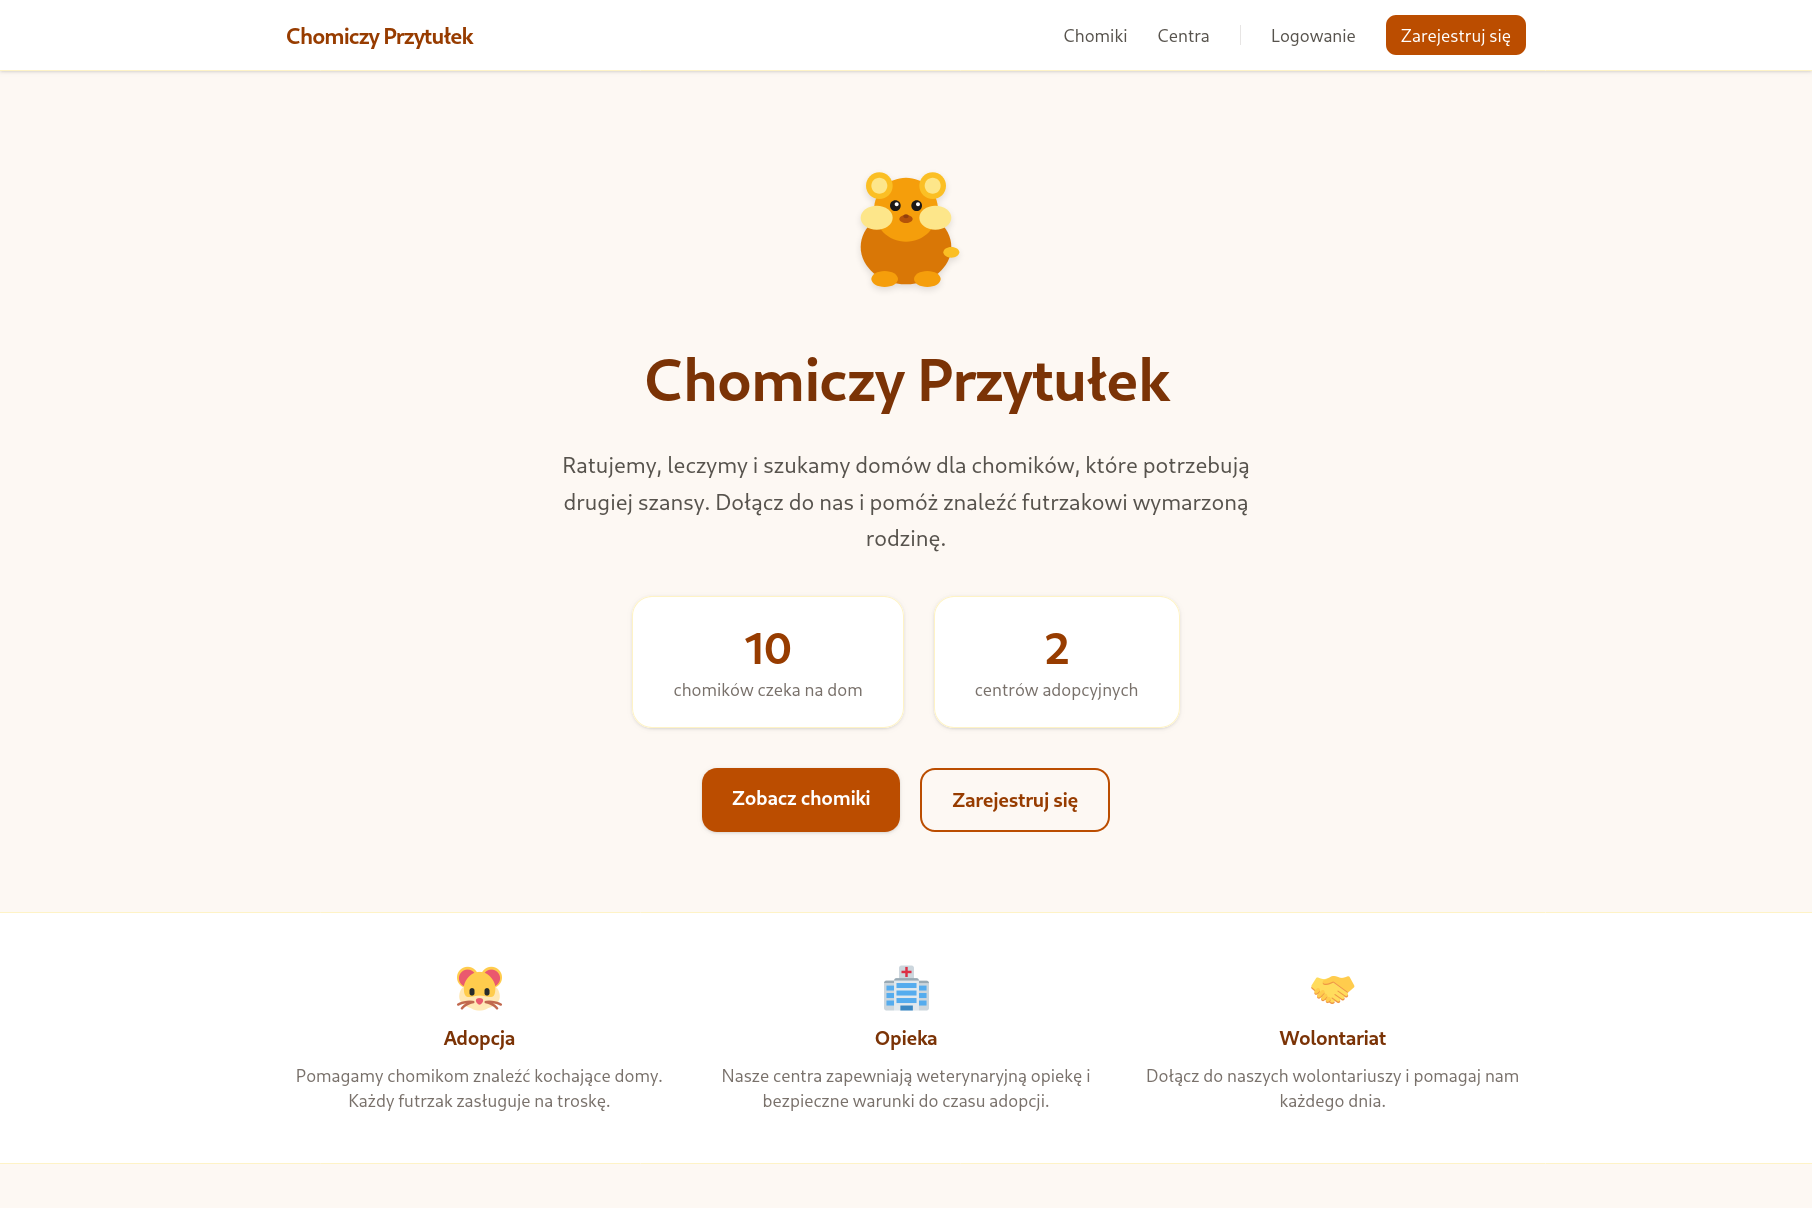
\includegraphics[height=\paperheight]{assets/homepage.png}%
    };
  \end{tikzpicture}
\end{frame}

% ── Slide 1 ──────────────────────────────────────────────────────────────────
\begin{frame}
  \frametitle{Stowarzyszenie Pomocy Chomikom}
  \begin{columns}[c]
    \column{0.5\textwidth}
      \centering
      
\includegraphics[width=\linewidth, height=0.78\textheight, keepaspectratio]{assets/kroliki_krakow.jpg}
    \column{0.5\textwidth}
      \centering
      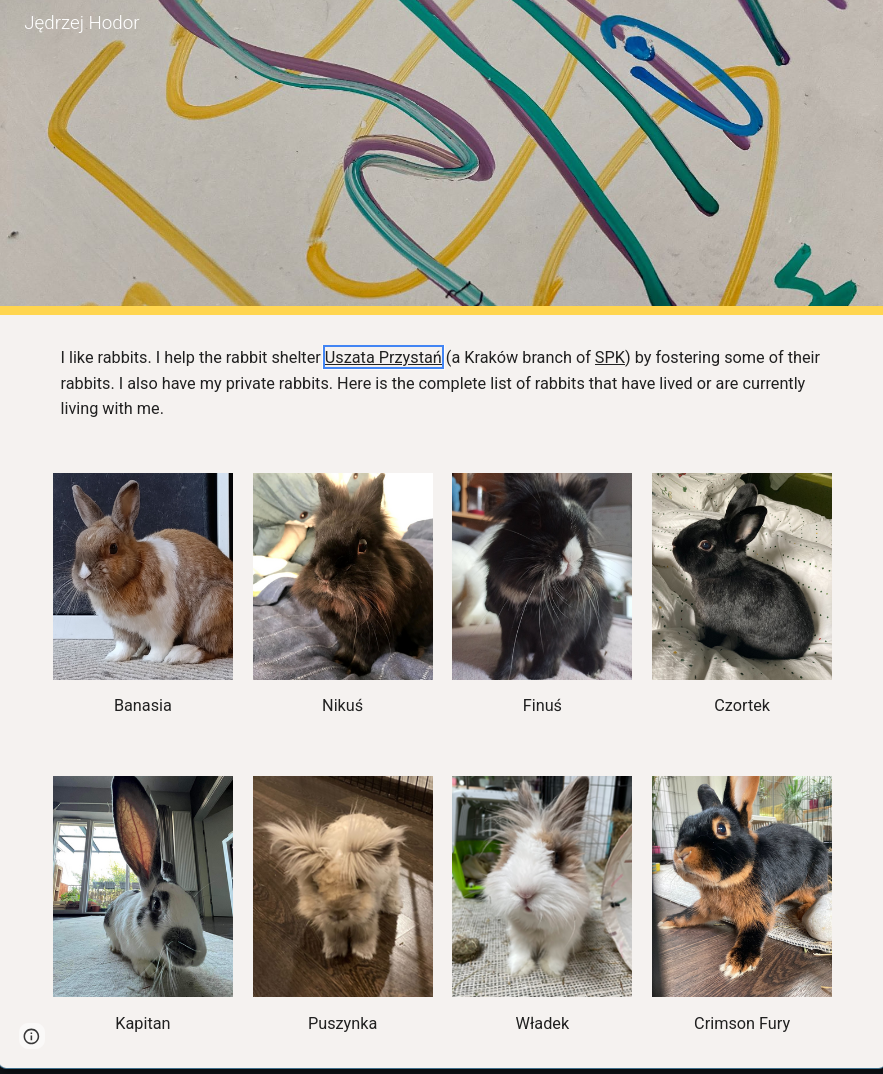
\includegraphics[width=\linewidth, height=0.78\textheight, keepaspectratio]{assets/hodor.png}
  \end{columns}
\end{frame}

% ── Slide 2 ──────────────────────────────────────────────────────────────────
\begin{frame}[plain]
  \fullslideimage{assets/schema.png}
\end{frame}

% ── Slide 3a ─────────────────────────────────────────────────────────────────
\begin{frame}
  \frametitle{Wolontariusze}
  \centering
  
\includegraphics[width=\linewidth, height=0.82\textheight, keepaspectratio]{assets/volunteers.png}
\end{frame}

% ── Slide 3b ─────────────────────────────────────────────────────────────────
\begin{frame}
  \frametitle{Adopcje}
  \centering
  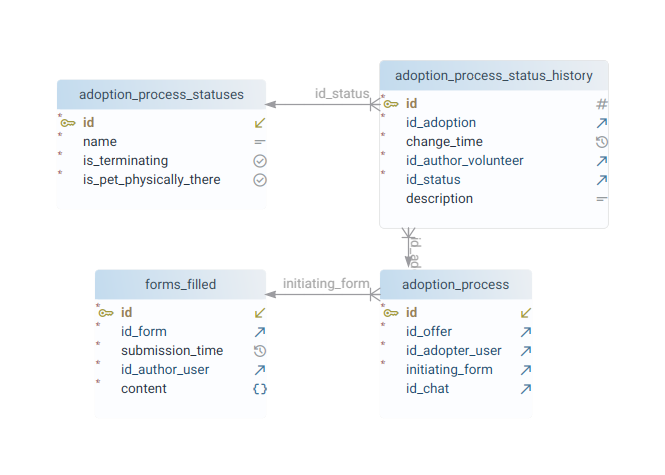
\includegraphics[width=\linewidth, height=0.82\textheight, keepaspectratio]{assets/adoptions.png}
\end{frame}

% ── Slide 4 ──────────────────────────────────────────────────────────────────
\begin{frame}
  \frametitle{Gatunki chomików}
  \centering
  
\includegraphics[width=1\linewidth, height=0.7\textheight, keepaspectratio]{assets/species.png}\\[0.5em]
  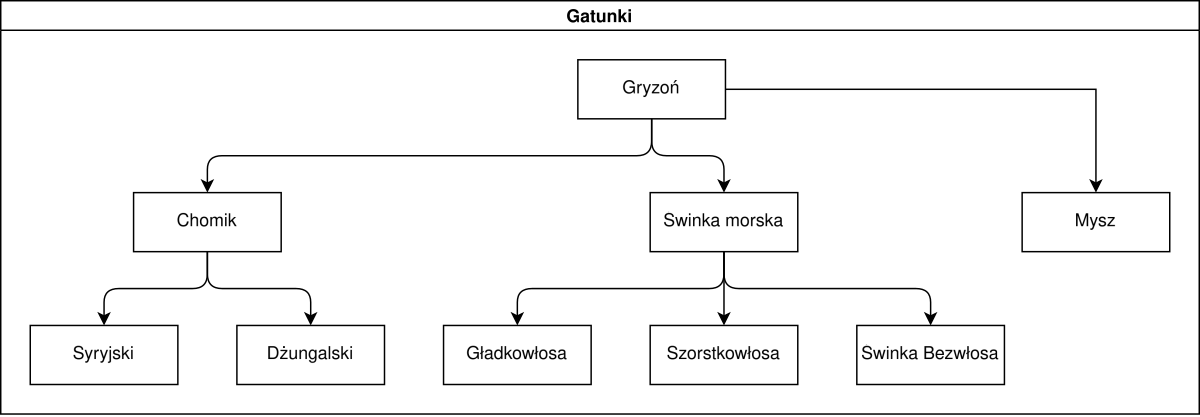
\includegraphics[width=1\linewidth, height=0.5\textheight, keepaspectratio]{assets/species_tree.png}
\end{frame}

% ── Slide 5 ──────────────────────────────────────────────────────────────────
\begin{frame}[plain]
  \fullslideimage{assets/zig.png}
\end{frame}

\begin{frame}{Analiza Wydajności Platformy}
    \begin{center}
        \begin{tikzpicture}
            % --- PARAMETRY DO MODYFIKACJI ---
            \pgfmathsetmacro{\barWidth}{1.5}      % Szerokość słupka
            \pgfmathsetmacro{\barGap}{2}        % Odstęp między słupkami
            \pgfmathsetmacro{\ourHeight}{4.5}     % Wysokość naszego słupka (chomiki)
            \pgfmathsetmacro{\compHeight}{0.4}    % Wysokość konkurencji
            \pgfmathsetmacro{\axisExt}{0.5}       % O ile oś wystaje ponad najwyższy słupek
            
            % Definicja kolorów (jeśli nie masz ich w preambule)
            \definecolor{accentColor}{HTML}{B45309} % Twoje brązowe akcenty
            
            % --- OBLICZENIA AUTOMATYCZNE ---
            \pgfmathsetmacro{\totalAxisH}{\ourHeight + \axisExt}
            \pgfmathsetmacro{\ourX}{\barGap + \barWidth/2}
            \pgfmathsetmacro{\compX}{0}
            \pgfmathsetmacro{\textY}{\ourHeight + 1}
            
            % Oś pionowa
            \draw[->, thick] (-0.5,0) -- (-0.5, \totalAxisH) 
                node[above, rotate=90, midway, yshift=0.6cm] {chomiki na sekundę [ch/s]};
            
            % Słupek Konkurencji
            \fill[gray!30] (\compX, 0) rectangle ++(\barWidth, \compHeight);
            \node[below, text=gray] at (\compX + \barWidth/2, -0.1) {Konkurencja};
            \node[above, gray, font=\tiny] at (\compX + \barWidth/2, \compHeight) {smutek};
            
            % Nasz Słupek
            \fill[accentColor] (\ourX, 0) rectangle ++(\barWidth, \ourHeight);
            \node[below, font=\bfseries, color=accentColor] at (\ourX + \barWidth/2, -0.1) {Nasza platforma};
            \node[above, font=\bfseries, color=accentColor] at (\ourX + \barWidth/2, \ourHeight) {MOC};
            
            % Dynamiczny napis 10x
            \node at (0.5*\ourX + 0.5*\barWidth, \textY) {\Huge \textbf{\color{accentColor} 10x}};
            
            % Linia bazowa (oś X)
            \draw[thick] (-0.7,0) -- (\ourX + \barWidth + 0.5, 0);

            % Humorystyczna stopka
            \node[anchor=north east, font=\tiny, gray] at (\ourX + \barWidth, -0.8) 
                {* Dane oparte na liczbie obrotów kołowrotka.};
        \end{tikzpicture}
    \end{center}
\end{frame}

% ── Slide 6 ──────────────────────────────────────────────────────────────────
\begin{frame}[plain]
  \fullslideimage{assets/qr.png}
\end{frame}

\end{document}
